\section{Deep and shallow semantic construction}
\label{sec:motivation}

% Motivate what we're doing and provide background.  Example outputs of
% deep and shallow parsers.  Illustrate and state the problem.
%
% Try to find an eg where the comparison isn't easy to see (from Anna
% Ritchie's deliverable?). 
% NOTE: on Ritichie: Perhaps "Three dogs bark on Tuesday in
% June" from page 11?  It's hard to follow what's going on, from the
% sheer size of the RMRSs and the need to allow for variation on the
% variable names.  But I don't know how to extract this figure
% techinically; nor whether we have room.

We motivate and describe {\sc rmrs} with a toy
example.  Sentence 
(\ref{eg:cat}a) features a semantic scope ambiguity that, according to
most deep grammars, syntax
doesn't resolve.    The {\sc mrs} (\ref{eg:cat}b) derived by the
{\sc erg} \cite{copestake:flickinger:2000}
reflects this: (i) each predication is
labelled ($l_1$, $l_4$, etc); (ii) scopal arguments are indicated by
holes (e.g., $h_2$, $h_3$); (iii)
constraints on scope are expressed by the qeq conditions (roughly, $h
=_q l$ means that only zero or more quantifiers lie between the scopal
argument $h$ and the predication labelled by $l$ in any fully-resolved
logical form); and (iv) these scope
constraints allow for more than one way of `plugging' the holes with
labels.\footnote{The event variable in $\_\mbox{{\em fat}}\_j\_1$ is 
  for copulas. {\em The
    cat is fat} has logical form 
  $\mbox{\_the\_q\_1}(x,\mbox{\_cat\_n\_1}(x),\mbox{\_fat\_j\_1}(e,x))$.}
\begin{examples}
\item   \label{eg:cat}
\begin{subexamples}
\item
Every fat cat chased some dog.
% \item
% $\mbox{\_every\_q\_1}(x, \mbox{\_fat\_j\_1}(e',x) \wedge
% \mbox{\_cat\_n\_1}(x),$\\
% \hspace*{0.5in}$\mbox{\_some\_q\_1}(y, \mbox{\_dog\_n\_1}(y),
% \mbox{\_chase\_v\_1}(e_{spast},x) )$\\
% $\mbox{\_some\_q\_1}(y, \mbox{\_dog\_n\_1}(y),$\\
% \hspace*{0.5in}$\mbox{\_every\_q\_1}(x, \mbox{\_fat\_j\_1}(e',x)
% \wedge 
% \mbox{\_cat\_n\_1}(x), 
% \mbox{\_chase\_v\_1}(e_{spast},x)))$
\item   $l_1\handel\mbox{\_every\_q\_1}(x,h_2,h_3)$\\
$l_4\handel\mbox{\_fat\_j\_1}(e',x)$\\
$l_4\handel\mbox{\_cat\_n\_1}(x)$\\
$l_5\handel\mbox{\_chased\_n\_1}(e,x,y)$\\
$l_6\handel\mbox{\_some\_n\_1}(y,h_7,h_8)$\\
$l_9\handel\mbox{\_dog\_n\_1}(y)$\\
$h_2 =_q l_4, h_7 =_q l_9$
\end{subexamples}
\end{examples}
(\ref{eg:cat}b) also exhibits {\sc mrs}' compact description of
conjunction through label sharing (see $l_4$), and the {\sc
  erg}'s naming convention for predicate symbols: each lexical predicate is
constructed from the word lemma, its syntactic category and a sense
number, and the leading underscore distinguishes lexical predicates
from non-lexical ones.

Conceptually, this {\sc mrs} is a partial description of all its
possible (fully specific) interpretations in context.  
These are expressed in a so-called {\em base language}, where each
predicate symbol in the {\sc mrs} is a proxy for one or more
base-language constructors of the same arity.
Assuming a very close
correspondence between the {\sc mrs} predicate symbols and the
base-language constructors they 
stand for, the {\sc mrs}
(\ref{eg:cat}b) (partially) describes both the base-language formulae in
Figure~\ref{fig:1}, shown as trees to emphasise that an {\sc mrs} is a
partial description of the formulae's {\em form}; not its
(base-language) entailments. 
In essence, the labels in the {\sc mrs} reify the
nodes in the tree, and each of these trees encodes one way of equating
holes with labels that respects qeq constraints and binding conditions
on the variables.

\begin{figure}[h]

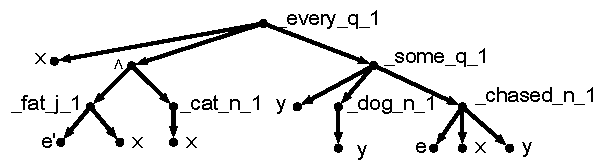
\includegraphics[width=6cm]{pic-cat-chased-dog}

Put trees in here

\caption{The Form of alternative base logical forms of
  (\ref{eg:cat}a).}
\label{fig:1}
\end{figure}

The {\sc mrs} (\ref{eg:cat}b) is a notational variant of the {\sc
  rmrs} (\ref{eg:cat}c). {\sc rmrs}s offer a more factorised
representation: each predicate symbol is unary and the other
arguments to its corresonding base-language constructor
are represented by separate binary relations on the unique {\em
  anchor} of the predicate symbol ($a_1, a_{41},\ldots$) together with
variable equalities (e.g., $x=x_1$).
\begin{examples}
\item   [\ref{eg:cat}]
\begin{subexamples}
\item   [c]
$l_1:a_1\handel\mbox{\_every\_q\_1}(x_1),$\\
\hspace*{0.1in}$\mbox{RSTR}(a_1,h_2),
\mbox{BODY}(a_1,h_3)$\\ 
$l_{41}:a_{41}\handel\mbox{\_fat\_j\_1}(e'), \mbox{ARG1}(a_{41},x_2)$\\
$l_{42}:a_{42}\handel\mbox{\_cat\_n\_1}(x_3)$\\
$l_5:a_5\handel\mbox{\_chase\_v\_1}(e_{spast})$,\\
\hspace*{0.1in}$\mbox{ARG1}(a_5,x_4),
\mbox{ARG2}(a_5,x_5)$\\ 
$l_6:a_6\handel\mbox{\_some\_q\_1}(x_6)$,\\
\hspace*{0.1in}$\mbox{RSTR}(a_6,h_7),
\mbox{BODY}(a_6,h_8)$\\ 
$l_9:a_9\handel\mbox{\_dog\_n\_1}(x_7)$\\
$h_2=_q l_{42}, l_{41}=l_{42}, h_7 =_q l_9$\\
$x_1=x_2, x_2=x_3, x_3=x_4,$\\
$x_5=x_6, x_5=x_7$
\end{subexamples}
\end{examples}

This factored representation allows one to build semantic components
to shallow parsers where lexical or syntactic information is absent.
An extreme example would be a {\sc 
  pos} tagger: one can build its semantic component simply by deriving
lexical predicate symbols from the word lemmas and tags and assigning each
predication a unique label, anchor and
argument, as in (\ref{eg:cat-pos}):
\begin{examples}
\item   \label{eg:cat-pos}
\begin{subexamples}
\item   Every\_{\sc at1} fat\_{\sc jj} cat\_{\sc nn1} chased\_{\sc
    vvd} some\_{\sc dd} dog\_{\sc nn1}
\item   $l_1:a_1:\mbox{\_every\_q}(x)$, \\
$l_{41}:a_{41}:\mbox{\_fat\_a}(e')$,\\
$l_{42}:a_{42}:\mbox{\_cat\_n}(x_3)$\\
$l_5:a_5:\mbox{\_chased\_v}(e_{past})$, \\
$l_6:a_6:\mbox{\_some\_q}(x_4)$, \\
$l_9:a_9:\mbox{\_dog\_n}(x_5)$
\end{subexamples}
\end{examples}

Semantic relations, sense tags and the arity of the base-language
constructors are
missing from (\ref{eg:cat-pos}b) because the {\sc pos} tagger doesn't
reveal information about syntactic constituency, word sense or lexical
subcategorisation respectively.  
But the {\sc rmrs}s (\ref{eg:cat}c) and
(\ref{eg:cat-pos}b) are entirely compatible, the former being more
specific than the latter.  At least, this holds so long as the
base-language constructors that the {\sc rmrs} predicate symbol
{\_name\_t\_s} corresponds to is a 
subset of those corresponding to the predicate symbol {\em \_name\_t},
for any word lemma {\em name}, {\sc pos} tag $t$ and sense $s$ (written 
$\mbox{{\em \_name\_t\_s}} \sqsubset \mbox{{\em name\_t}}$). 

The values of non-scopal arguments are underspecified through the
absence of ARG relations and/or through the absence of
equalities and inequalities among the variables $x_1, x_2,\ldots$.
The need to
underspecify such semantic dependencies is required when
the shallow parser doesn't record syntactic dependencies.
Indeed, there is no single {\sc mrs} which is satisfied by both the
trees in Figure~\ref{fig:2}, assuming of course that disjunction is not part of
the {\sc mrs} language.  In words, these trees collectively specify
the (partial) semantic information that $x$ is either the second
argument (i.e., the direct object) or the third argument (i.e., the
indirect object) to {\em give}, but we don't know which.  
A shallow
processor that misses long distance dependencies in
(\ref{eg:which-dog}) cannot
discern that the bone is the second argument to {\em
  give} in (\ref{eg:which-dog}a), while the dog is the third argument
in (\ref{eg:which-dog}b).
\begin{examples}
\item   \label{eg:which-dog}
\begin{subexamples}
\item   To which dog did Kim give the bone?
\item   Which bone did Kim give the dog?
\end{subexamples}
\end{examples}
Thus to maximise the semantic contribution
of the parser while not overdetermining it, the phrases
{\em give the bone} vs.\
{\em give the dog} should whether the semantic index of the noun
phrase is the second or third argument to {\em give},
as shown in Figure~\ref{fig:2}.   This will be expressed in
{\sc rmrs} via the binary relation  $\mbox{{\em ARG}}_{\{2,3\}}(a,x)$
between the anchor $a$ of the predicate symbol for {\em give} and the
individual $x$.   More generally, $\mbox{{\em ARG}}_n(a,x)$ means that
$x$ is an argument to the predicate anchored at $a$, but its argument
position is unspecified.

\begin{figure}

\leaf{$e$}
\leaf{$\ldots$}
\leaf{$x$}
\leaf{$\ldots$}
\branch{4}{\_give\_v\_b1}
\tree
\hfill
\leaf{$e$}
\leaf{$\ldots$}
\leaf{$\ldots$}
\leaf{$x$}
\branch{4}{\_give\_v\_b1}
\tree

\caption{$x$ is a participant in a
  giving event, but $x$'s role is unknown.}
\label{fig:2}
\end{figure}

The binary ARG relations also supports underspecifying the {\em arity}
of the base-language constructors, as is required when lexical
subcategorisation information is missing from the shallow parser.
While a deep parser assumes complete information about lexical
subcategorisation in any of its derivations, thereby fixing the arity
of the base-language constructors in the fully-specific logical form
to be the same as the {\sc mrs} predicate symbol $P$ that's introduced by
the lexeme, the predicate symbols in an {\sc rmrs} yielded from a
shallow parse should, in principle at least,
correspond to base language constructors of mixed arity.  For
instance, the English verb {\em bake} can be used causatively ({\em
  Kim baked the potatoes}), in which case semantically it corresponds
to a 3-place predicate symbol {\em \_bake\_v\_b1} in the base
language, or it may be used 
inchoatively ({\em the potatoes are baking}), that semantically
corresponds to a 2-place predicate {\em \_bake\_v\_b2}.  So the 
predicate symbol {\em 
  \_bake\_v} in the {\sc rmrs} that's introduced by a {\sc pos} tagger
must be able to denote either of these
base-language predicates in the {\sc rmrs}'s interpretation.

\hidden{
Finally, {\sc rmrs} allows one to underspecify the {\em sort} of an
argument by including in its language meta-variables $u_1,u_2,\ldots$
over individual, event, and handle variables.  For instance, the predicate
symbol {\em \_be\_v} produced by a {\sc pos} tagger is resolvable to several
3-place base-language constructors whose argument-types 
vary: the base-language constructor corresponding
to its use in {\em John is a man} takes an event and two individuals
as arguments; but in {\em It is John who talked} the constructor takes
an event, an individual and a proposition as arguments.
}


%%% Local Variables: 
%%% mode: latex
%%% TeX-master: "rmrs-08"
%%% End: 
